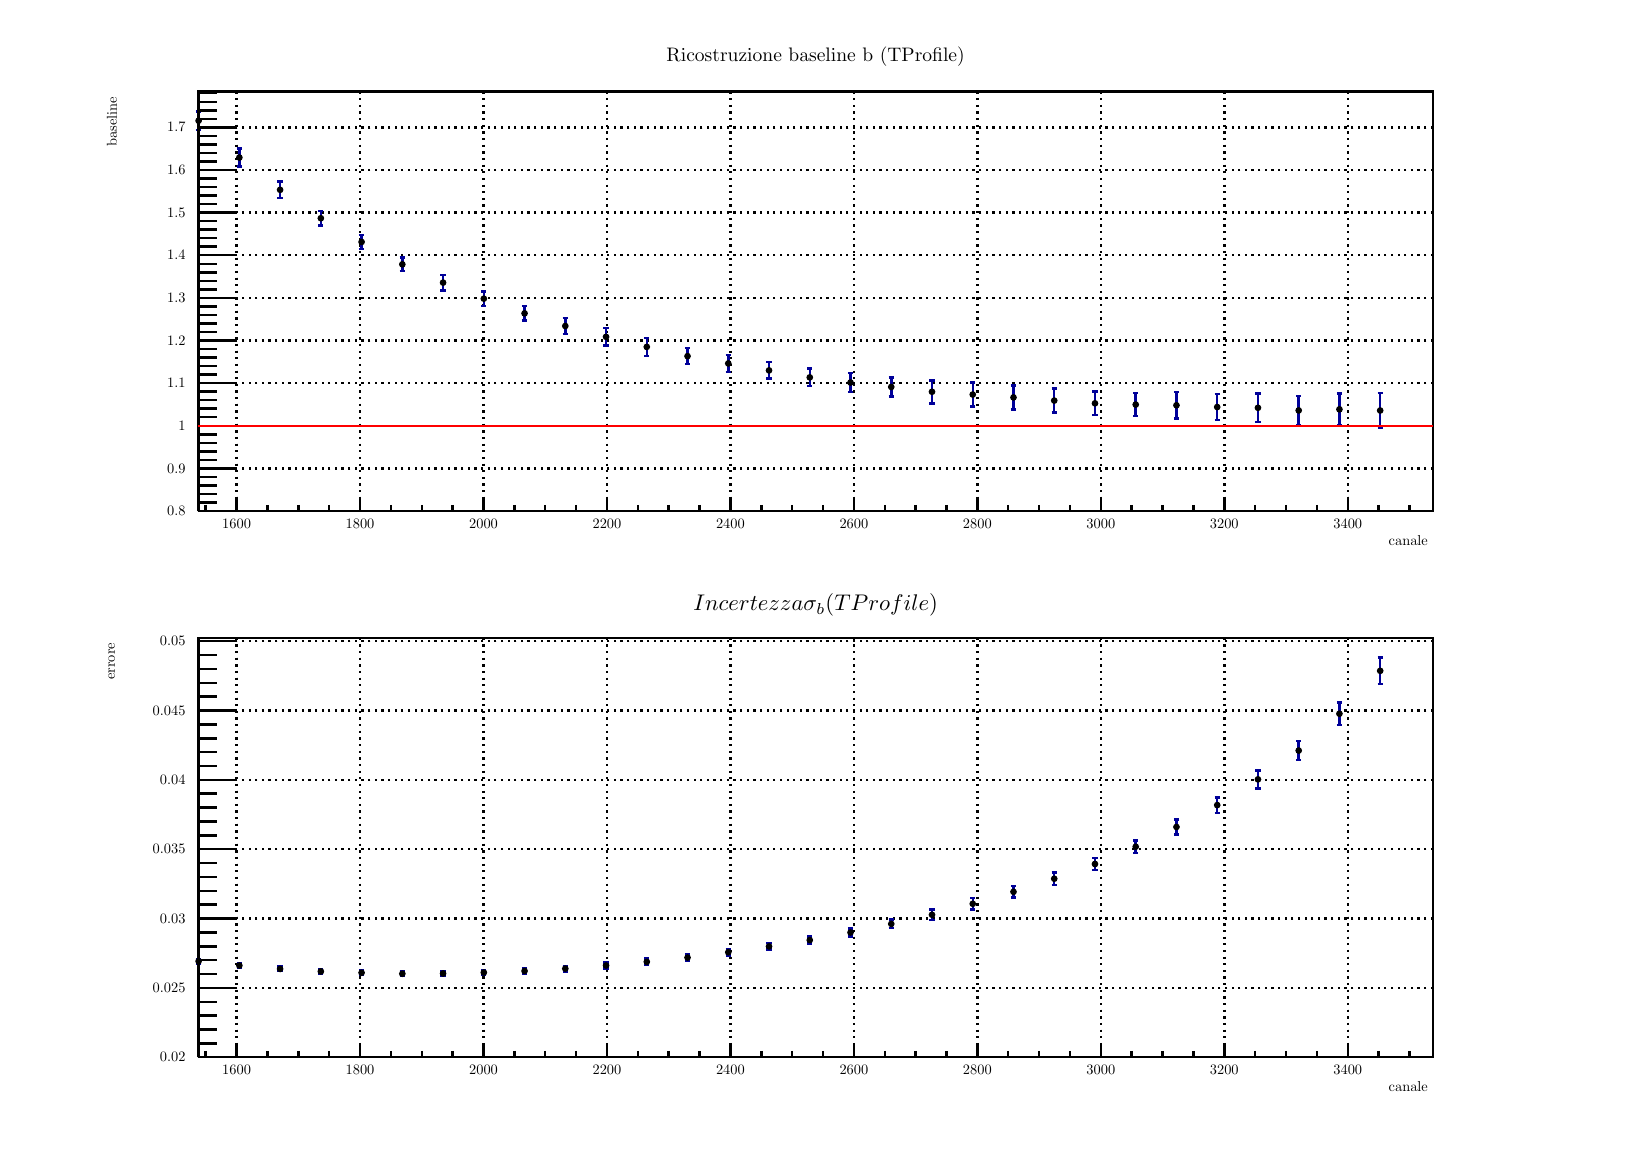
\begin{tikzpicture}
\pgfdeclareplotmark{cross} {
\pgfpathmoveto{\pgfpoint{-0.3\pgfplotmarksize}{\pgfplotmarksize}}
\pgfpathlineto{\pgfpoint{+0.3\pgfplotmarksize}{\pgfplotmarksize}}
\pgfpathlineto{\pgfpoint{+0.3\pgfplotmarksize}{0.3\pgfplotmarksize}}
\pgfpathlineto{\pgfpoint{+1\pgfplotmarksize}{0.3\pgfplotmarksize}}
\pgfpathlineto{\pgfpoint{+1\pgfplotmarksize}{-0.3\pgfplotmarksize}}
\pgfpathlineto{\pgfpoint{+0.3\pgfplotmarksize}{-0.3\pgfplotmarksize}}
\pgfpathlineto{\pgfpoint{+0.3\pgfplotmarksize}{-1.\pgfplotmarksize}}
\pgfpathlineto{\pgfpoint{-0.3\pgfplotmarksize}{-1.\pgfplotmarksize}}
\pgfpathlineto{\pgfpoint{-0.3\pgfplotmarksize}{-0.3\pgfplotmarksize}}
\pgfpathlineto{\pgfpoint{-1.\pgfplotmarksize}{-0.3\pgfplotmarksize}}
\pgfpathlineto{\pgfpoint{-1.\pgfplotmarksize}{0.3\pgfplotmarksize}}
\pgfpathlineto{\pgfpoint{-0.3\pgfplotmarksize}{0.3\pgfplotmarksize}}
\pgfpathclose
\pgfusepathqstroke
}
\pgfdeclareplotmark{cross*} {
\pgfpathmoveto{\pgfpoint{-0.3\pgfplotmarksize}{\pgfplotmarksize}}
\pgfpathlineto{\pgfpoint{+0.3\pgfplotmarksize}{\pgfplotmarksize}}
\pgfpathlineto{\pgfpoint{+0.3\pgfplotmarksize}{0.3\pgfplotmarksize}}
\pgfpathlineto{\pgfpoint{+1\pgfplotmarksize}{0.3\pgfplotmarksize}}
\pgfpathlineto{\pgfpoint{+1\pgfplotmarksize}{-0.3\pgfplotmarksize}}
\pgfpathlineto{\pgfpoint{+0.3\pgfplotmarksize}{-0.3\pgfplotmarksize}}
\pgfpathlineto{\pgfpoint{+0.3\pgfplotmarksize}{-1.\pgfplotmarksize}}
\pgfpathlineto{\pgfpoint{-0.3\pgfplotmarksize}{-1.\pgfplotmarksize}}
\pgfpathlineto{\pgfpoint{-0.3\pgfplotmarksize}{-0.3\pgfplotmarksize}}
\pgfpathlineto{\pgfpoint{-1.\pgfplotmarksize}{-0.3\pgfplotmarksize}}
\pgfpathlineto{\pgfpoint{-1.\pgfplotmarksize}{0.3\pgfplotmarksize}}
\pgfpathlineto{\pgfpoint{-0.3\pgfplotmarksize}{0.3\pgfplotmarksize}}
\pgfpathclose
\pgfusepathqfillstroke
}
\pgfdeclareplotmark{newstar} {
\pgfpathmoveto{\pgfqpoint{0pt}{\pgfplotmarksize}}
\pgfpathlineto{\pgfqpointpolar{44}{0.5\pgfplotmarksize}}
\pgfpathlineto{\pgfqpointpolar{18}{\pgfplotmarksize}}
\pgfpathlineto{\pgfqpointpolar{-20}{0.5\pgfplotmarksize}}
\pgfpathlineto{\pgfqpointpolar{-54}{\pgfplotmarksize}}
\pgfpathlineto{\pgfqpointpolar{-90}{0.5\pgfplotmarksize}}
\pgfpathlineto{\pgfqpointpolar{234}{\pgfplotmarksize}}
\pgfpathlineto{\pgfqpointpolar{198}{0.5\pgfplotmarksize}}
\pgfpathlineto{\pgfqpointpolar{162}{\pgfplotmarksize}}
\pgfpathlineto{\pgfqpointpolar{134}{0.5\pgfplotmarksize}}
\pgfpathclose
\pgfusepathqstroke
}
\pgfdeclareplotmark{newstar*} {
\pgfpathmoveto{\pgfqpoint{0pt}{\pgfplotmarksize}}
\pgfpathlineto{\pgfqpointpolar{44}{0.5\pgfplotmarksize}}
\pgfpathlineto{\pgfqpointpolar{18}{\pgfplotmarksize}}
\pgfpathlineto{\pgfqpointpolar{-20}{0.5\pgfplotmarksize}}
\pgfpathlineto{\pgfqpointpolar{-54}{\pgfplotmarksize}}
\pgfpathlineto{\pgfqpointpolar{-90}{0.5\pgfplotmarksize}}
\pgfpathlineto{\pgfqpointpolar{234}{\pgfplotmarksize}}
\pgfpathlineto{\pgfqpointpolar{198}{0.5\pgfplotmarksize}}
\pgfpathlineto{\pgfqpointpolar{162}{\pgfplotmarksize}}
\pgfpathlineto{\pgfqpointpolar{134}{0.5\pgfplotmarksize}}
\pgfpathclose
\pgfusepathqfillstroke
}
\definecolor{c}{rgb}{1,1,1};
\draw [color=c, fill=c] (0,0) rectangle (20,13.8731);
\draw [color=c, fill=c] (0.2,7.07529) rectangle (19.8,13.7344);
\draw [color=c, fill=c] (2.16,7.7412) rectangle (17.84,13.0685);
\definecolor{c}{rgb}{0,0,0};
\draw [c,line width=0.9] (2.16,7.7412) -- (2.16,13.0685) -- (17.84,13.0685) -- (17.84,7.7412) -- (2.16,7.7412);
\definecolor{c}{rgb}{1,1,1};
\draw [color=c, fill=c] (2.16,7.7412) rectangle (17.84,13.0685);
\definecolor{c}{rgb}{0,0,0};
\draw [c,line width=0.9] (2.16,7.7412) -- (2.16,13.0685) -- (17.84,13.0685) -- (17.84,7.7412) -- (2.16,7.7412);
\draw [c,line width=0.9] (2.16,7.7412) -- (17.84,7.7412);
\draw [c,dash pattern=on 0.80pt off 1.60pt ,line width=0.9] (2.64608,13.0685) -- (2.64608,7.7412);
\draw [c,dash pattern=on 0.80pt off 1.60pt ,line width=0.9] (4.21408,13.0685) -- (4.21408,7.7412);
\draw [c,dash pattern=on 0.80pt off 1.60pt ,line width=0.9] (5.78208,13.0685) -- (5.78208,7.7412);
\draw [c,dash pattern=on 0.80pt off 1.60pt ,line width=0.9] (7.35008,13.0685) -- (7.35008,7.7412);
\draw [c,dash pattern=on 0.80pt off 1.60pt ,line width=0.9] (8.91808,13.0685) -- (8.91808,7.7412);
\draw [c,dash pattern=on 0.80pt off 1.60pt ,line width=0.9] (10.4861,13.0685) -- (10.4861,7.7412);
\draw [c,dash pattern=on 0.80pt off 1.60pt ,line width=0.9] (12.0541,13.0685) -- (12.0541,7.7412);
\draw [c,dash pattern=on 0.80pt off 1.60pt ,line width=0.9] (13.6221,13.0685) -- (13.6221,7.7412);
\draw [c,dash pattern=on 0.80pt off 1.60pt ,line width=0.9] (15.1901,13.0685) -- (15.1901,7.7412);
\draw [c,dash pattern=on 0.80pt off 1.60pt ,line width=0.9] (16.7581,13.0685) -- (16.7581,7.7412);
\draw [c,dash pattern=on 0.80pt off 1.60pt ,line width=0.9] (2.64608,13.0685) -- (2.64608,7.7412);
\draw [c,dash pattern=on 0.80pt off 1.60pt ,line width=0.9] (16.7581,13.0685) -- (16.7581,7.7412);
\draw [c,line width=0.9] (2.16,7.7412) -- (2.16,13.0685);
\draw [c,dash pattern=on 0.80pt off 1.60pt ,line width=0.9] (17.84,7.7412) -- (2.16,7.7412);
\draw [c,dash pattern=on 0.80pt off 1.60pt ,line width=0.9] (17.84,8.28265) -- (2.16,8.28265);
\draw [c,dash pattern=on 0.80pt off 1.60pt ,line width=0.9] (17.84,8.82409) -- (2.16,8.82409);
\draw [c,dash pattern=on 0.80pt off 1.60pt ,line width=0.9] (17.84,9.36554) -- (2.16,9.36554);
\draw [c,dash pattern=on 0.80pt off 1.60pt ,line width=0.9] (17.84,9.90699) -- (2.16,9.90699);
\draw [c,dash pattern=on 0.80pt off 1.60pt ,line width=0.9] (17.84,10.4484) -- (2.16,10.4484);
\draw [c,dash pattern=on 0.80pt off 1.60pt ,line width=0.9] (17.84,10.9899) -- (2.16,10.9899);
\draw [c,dash pattern=on 0.80pt off 1.60pt ,line width=0.9] (17.84,11.5313) -- (2.16,11.5313);
\draw [c,dash pattern=on 0.80pt off 1.60pt ,line width=0.9] (17.84,12.0728) -- (2.16,12.0728);
\draw [c,dash pattern=on 0.80pt off 1.60pt ,line width=0.9] (17.84,12.6142) -- (2.16,12.6142);
\draw [c,dash pattern=on 0.80pt off 1.60pt ,line width=0.9] (17.84,12.6142) -- (2.16,12.6142);
\definecolor{c}{rgb}{0,0,0.6};
\draw [c,line width=0.9] (2.16392,12.5823) -- (2.16392,12.6986);
\draw [c,line width=0.9] (2.16392,12.6986) -- (2.16392,12.8148);
\draw [c,line width=0.9] (2.16,12.6986) -- (2.16392,12.6986);
\draw [c,line width=0.9] (2.16392,12.6986) -- (2.16784,12.6986);
\draw [c,line width=0.9] (2.13053,12.5823) -- (2.19731,12.5823);
\draw [c,line width=0.9] (2.13053,12.8148) -- (2.19731,12.8148);
\draw [c,line width=0.9] (2.16,12.6652) -- (2.16,12.732);
\draw [c,line width=0.9] (2.16784,12.6652) -- (2.16784,12.732);
\definecolor{c}{rgb}{0,0,0};
\foreach \P in {(2.16392,12.6986)}{\draw[mark options={color=c,fill=c},mark size=2.402402pt,mark=*,mark size=1pt] plot coordinates {\P};}
\definecolor{c}{rgb}{0,0,0.6};
\draw [c,line width=0.9] (2.68136,12.1143) -- (2.68136,12.2306);
\draw [c,line width=0.9] (2.68136,12.2306) -- (2.68136,12.347);
\draw [c,line width=0.9] (2.67744,12.2306) -- (2.68136,12.2306);
\draw [c,line width=0.9] (2.68136,12.2306) -- (2.68528,12.2306);
\draw [c,line width=0.9] (2.64797,12.1143) -- (2.71475,12.1143);
\draw [c,line width=0.9] (2.64797,12.347) -- (2.71475,12.347);
\draw [c,line width=0.9] (2.67744,12.1972) -- (2.67744,12.264);
\draw [c,line width=0.9] (2.68528,12.1972) -- (2.68528,12.264);
\definecolor{c}{rgb}{0,0,0};
\foreach \P in {(2.68136,12.2306)}{\draw[mark options={color=c,fill=c},mark size=2.402402pt,mark=*,mark size=1pt] plot coordinates {\P};}
\definecolor{c}{rgb}{0,0,0.6};
\draw [c,line width=0.9] (3.1988,11.7148) -- (3.1988,11.8205);
\draw [c,line width=0.9] (3.1988,11.8205) -- (3.1988,11.9261);
\draw [c,line width=0.9] (3.19488,11.8205) -- (3.1988,11.8205);
\draw [c,line width=0.9] (3.1988,11.8205) -- (3.20272,11.8205);
\draw [c,line width=0.9] (3.16541,11.7148) -- (3.23219,11.7148);
\draw [c,line width=0.9] (3.16541,11.9261) -- (3.23219,11.9261);
\draw [c,line width=0.9] (3.19488,11.7871) -- (3.19488,11.8539);
\draw [c,line width=0.9] (3.20272,11.7871) -- (3.20272,11.8539);
\definecolor{c}{rgb}{0,0,0};
\foreach \P in {(3.1988,11.8205)}{\draw[mark options={color=c,fill=c},mark size=2.402402pt,mark=*,mark size=1pt] plot coordinates {\P};}
\definecolor{c}{rgb}{0,0,0.6};
\draw [c,line width=0.9] (3.71624,11.3669) -- (3.71624,11.46);
\draw [c,line width=0.9] (3.71624,11.46) -- (3.71624,11.5532);
\draw [c,line width=0.9] (3.71232,11.46) -- (3.71624,11.46);
\draw [c,line width=0.9] (3.71624,11.46) -- (3.72016,11.46);
\draw [c,line width=0.9] (3.68285,11.3669) -- (3.74963,11.3669);
\draw [c,line width=0.9] (3.68285,11.5532) -- (3.74963,11.5532);
\draw [c,line width=0.9] (3.71232,11.4267) -- (3.71232,11.4934);
\draw [c,line width=0.9] (3.72016,11.4267) -- (3.72016,11.4934);
\definecolor{c}{rgb}{0,0,0};
\foreach \P in {(3.71624,11.46)}{\draw[mark options={color=c,fill=c},mark size=2.402402pt,mark=*,mark size=1pt] plot coordinates {\P};}
\definecolor{c}{rgb}{0,0,0.6};
\draw [c,line width=0.9] (4.23368,11.0723) -- (4.23368,11.1586);
\draw [c,line width=0.9] (4.23368,11.1586) -- (4.23368,11.2449);
\draw [c,line width=0.9] (4.22976,11.1586) -- (4.23368,11.1586);
\draw [c,line width=0.9] (4.23368,11.1586) -- (4.2376,11.1586);
\draw [c,line width=0.9] (4.20029,11.0723) -- (4.26707,11.0723);
\draw [c,line width=0.9] (4.20029,11.2449) -- (4.26707,11.2449);
\draw [c,line width=0.9] (4.22976,11.1252) -- (4.22976,11.192);
\draw [c,line width=0.9] (4.2376,11.1252) -- (4.2376,11.192);
\definecolor{c}{rgb}{0,0,0};
\foreach \P in {(4.23368,11.1586)}{\draw[mark options={color=c,fill=c},mark size=2.402402pt,mark=*,mark size=1pt] plot coordinates {\P};}
\definecolor{c}{rgb}{0,0,0.6};
\draw [c,line width=0.9] (4.75112,10.7881) -- (4.75112,10.8742);
\draw [c,line width=0.9] (4.75112,10.8742) -- (4.75112,10.9603);
\draw [c,line width=0.9] (4.7472,10.8742) -- (4.75112,10.8742);
\draw [c,line width=0.9] (4.75112,10.8742) -- (4.75504,10.8742);
\draw [c,line width=0.9] (4.71773,10.7881) -- (4.78451,10.7881);
\draw [c,line width=0.9] (4.71773,10.9603) -- (4.78451,10.9603);
\draw [c,line width=0.9] (4.7472,10.8408) -- (4.7472,10.9076);
\draw [c,line width=0.9] (4.75504,10.8408) -- (4.75504,10.9076);
\definecolor{c}{rgb}{0,0,0};
\foreach \P in {(4.75112,10.8742)}{\draw[mark options={color=c,fill=c},mark size=2.402402pt,mark=*,mark size=1pt] plot coordinates {\P};}
\definecolor{c}{rgb}{0,0,0.6};
\draw [c,line width=0.9] (5.26856,10.544) -- (5.26856,10.6422);
\draw [c,line width=0.9] (5.26856,10.6422) -- (5.26856,10.7403);
\draw [c,line width=0.9] (5.26464,10.6422) -- (5.26856,10.6422);
\draw [c,line width=0.9] (5.26856,10.6422) -- (5.27248,10.6422);
\draw [c,line width=0.9] (5.23517,10.544) -- (5.30195,10.544);
\draw [c,line width=0.9] (5.23517,10.7403) -- (5.30195,10.7403);
\draw [c,line width=0.9] (5.26464,10.6088) -- (5.26464,10.6756);
\draw [c,line width=0.9] (5.27248,10.6088) -- (5.27248,10.6756);
\definecolor{c}{rgb}{0,0,0};
\foreach \P in {(5.26856,10.6422)}{\draw[mark options={color=c,fill=c},mark size=2.402402pt,mark=*,mark size=1pt] plot coordinates {\P};}
\definecolor{c}{rgb}{0,0,0.6};
\draw [c,line width=0.9] (5.786,10.3458) -- (5.786,10.4383);
\draw [c,line width=0.9] (5.786,10.4383) -- (5.786,10.5307);
\draw [c,line width=0.9] (5.78208,10.4383) -- (5.786,10.4383);
\draw [c,line width=0.9] (5.786,10.4383) -- (5.78992,10.4383);
\draw [c,line width=0.9] (5.75261,10.3458) -- (5.81939,10.3458);
\draw [c,line width=0.9] (5.75261,10.5307) -- (5.81939,10.5307);
\draw [c,line width=0.9] (5.78208,10.4049) -- (5.78208,10.4717);
\draw [c,line width=0.9] (5.78992,10.4049) -- (5.78992,10.4717);
\definecolor{c}{rgb}{0,0,0};
\foreach \P in {(5.786,10.4383)}{\draw[mark options={color=c,fill=c},mark size=2.402402pt,mark=*,mark size=1pt] plot coordinates {\P};}
\definecolor{c}{rgb}{0,0,0.6};
\draw [c,line width=0.9] (6.30344,10.1591) -- (6.30344,10.2517);
\draw [c,line width=0.9] (6.30344,10.2517) -- (6.30344,10.3444);
\draw [c,line width=0.9] (6.29952,10.2517) -- (6.30344,10.2517);
\draw [c,line width=0.9] (6.30344,10.2517) -- (6.30736,10.2517);
\draw [c,line width=0.9] (6.27005,10.1591) -- (6.33683,10.1591);
\draw [c,line width=0.9] (6.27005,10.3444) -- (6.33683,10.3444);
\draw [c,line width=0.9] (6.29952,10.2184) -- (6.29952,10.2851);
\draw [c,line width=0.9] (6.30736,10.2184) -- (6.30736,10.2851);
\definecolor{c}{rgb}{0,0,0};
\foreach \P in {(6.30344,10.2517)}{\draw[mark options={color=c,fill=c},mark size=2.402402pt,mark=*,mark size=1pt] plot coordinates {\P};}
\definecolor{c}{rgb}{0,0,0.6};
\draw [c,line width=0.9] (6.82088,9.99117) -- (6.82088,10.0913);
\draw [c,line width=0.9] (6.82088,10.0913) -- (6.82088,10.1915);
\draw [c,line width=0.9] (6.81696,10.0913) -- (6.82088,10.0913);
\draw [c,line width=0.9] (6.82088,10.0913) -- (6.8248,10.0913);
\draw [c,line width=0.9] (6.78749,9.99117) -- (6.85427,9.99117);
\draw [c,line width=0.9] (6.78749,10.1915) -- (6.85427,10.1915);
\draw [c,line width=0.9] (6.81696,10.058) -- (6.81696,10.1247);
\draw [c,line width=0.9] (6.8248,10.058) -- (6.8248,10.1247);
\definecolor{c}{rgb}{0,0,0};
\foreach \P in {(6.82088,10.0913)}{\draw[mark options={color=c,fill=c},mark size=2.402402pt,mark=*,mark size=1pt] plot coordinates {\P};}
\definecolor{c}{rgb}{0,0,0.6};
\draw [c,line width=0.9] (7.33832,9.84133) -- (7.33832,9.95353);
\draw [c,line width=0.9] (7.33832,9.95353) -- (7.33832,10.0657);
\draw [c,line width=0.9] (7.3344,9.95353) -- (7.33832,9.95353);
\draw [c,line width=0.9] (7.33832,9.95353) -- (7.34224,9.95353);
\draw [c,line width=0.9] (7.30493,9.84133) -- (7.37171,9.84133);
\draw [c,line width=0.9] (7.30493,10.0657) -- (7.37171,10.0657);
\draw [c,line width=0.9] (7.3344,9.92014) -- (7.3344,9.98692);
\draw [c,line width=0.9] (7.34224,9.92014) -- (7.34224,9.98692);
\definecolor{c}{rgb}{0,0,0};
\foreach \P in {(7.33832,9.95353)}{\draw[mark options={color=c,fill=c},mark size=2.402402pt,mark=*,mark size=1pt] plot coordinates {\P};}
\definecolor{c}{rgb}{0,0,0.6};
\draw [c,line width=0.9] (7.85576,9.71291) -- (7.85576,9.82609);
\draw [c,line width=0.9] (7.85576,9.82609) -- (7.85576,9.93928);
\draw [c,line width=0.9] (7.85184,9.82609) -- (7.85576,9.82609);
\draw [c,line width=0.9] (7.85576,9.82609) -- (7.85968,9.82609);
\draw [c,line width=0.9] (7.82237,9.71291) -- (7.88915,9.71291);
\draw [c,line width=0.9] (7.82237,9.93928) -- (7.88915,9.93928);
\draw [c,line width=0.9] (7.85184,9.7927) -- (7.85184,9.85948);
\draw [c,line width=0.9] (7.85968,9.7927) -- (7.85968,9.85948);
\definecolor{c}{rgb}{0,0,0};
\foreach \P in {(7.85576,9.82609)}{\draw[mark options={color=c,fill=c},mark size=2.402402pt,mark=*,mark size=1pt] plot coordinates {\P};}
\definecolor{c}{rgb}{0,0,0.6};
\draw [c,line width=0.9] (8.3732,9.60558) -- (8.3732,9.70828);
\draw [c,line width=0.9] (8.3732,9.70828) -- (8.3732,9.81098);
\draw [c,line width=0.9] (8.36928,9.70828) -- (8.3732,9.70828);
\draw [c,line width=0.9] (8.3732,9.70828) -- (8.37712,9.70828);
\draw [c,line width=0.9] (8.33981,9.60558) -- (8.40659,9.60558);
\draw [c,line width=0.9] (8.33981,9.81098) -- (8.40659,9.81098);
\draw [c,line width=0.9] (8.36928,9.67489) -- (8.36928,9.74167);
\draw [c,line width=0.9] (8.37712,9.67489) -- (8.37712,9.74167);
\definecolor{c}{rgb}{0,0,0};
\foreach \P in {(8.3732,9.70828)}{\draw[mark options={color=c,fill=c},mark size=2.402402pt,mark=*,mark size=1pt] plot coordinates {\P};}
\definecolor{c}{rgb}{0,0,0.6};
\draw [c,line width=0.9] (8.89064,9.51019) -- (8.89064,9.61603);
\draw [c,line width=0.9] (8.89064,9.61603) -- (8.89064,9.72186);
\draw [c,line width=0.9] (8.88672,9.61603) -- (8.89064,9.61603);
\draw [c,line width=0.9] (8.89064,9.61603) -- (8.89456,9.61603);
\draw [c,line width=0.9] (8.85725,9.51019) -- (8.92403,9.51019);
\draw [c,line width=0.9] (8.85725,9.72186) -- (8.92403,9.72186);
\draw [c,line width=0.9] (8.88672,9.58264) -- (8.88672,9.64942);
\draw [c,line width=0.9] (8.89456,9.58264) -- (8.89456,9.64942);
\definecolor{c}{rgb}{0,0,0};
\foreach \P in {(8.89064,9.61603)}{\draw[mark options={color=c,fill=c},mark size=2.402402pt,mark=*,mark size=1pt] plot coordinates {\P};}
\definecolor{c}{rgb}{0,0,0.6};
\draw [c,line width=0.9] (9.40808,9.42254) -- (9.40808,9.52749);
\draw [c,line width=0.9] (9.40808,9.52749) -- (9.40808,9.63244);
\draw [c,line width=0.9] (9.40416,9.52749) -- (9.40808,9.52749);
\draw [c,line width=0.9] (9.40808,9.52749) -- (9.412,9.52749);
\draw [c,line width=0.9] (9.37469,9.42254) -- (9.44147,9.42254);
\draw [c,line width=0.9] (9.37469,9.63244) -- (9.44147,9.63244);
\draw [c,line width=0.9] (9.40416,9.4941) -- (9.40416,9.56088);
\draw [c,line width=0.9] (9.412,9.4941) -- (9.412,9.56088);
\definecolor{c}{rgb}{0,0,0};
\foreach \P in {(9.40808,9.52749)}{\draw[mark options={color=c,fill=c},mark size=2.402402pt,mark=*,mark size=1pt] plot coordinates {\P};}
\definecolor{c}{rgb}{0,0,0.6};
\draw [c,line width=0.9] (9.92552,9.32941) -- (9.92552,9.43897);
\draw [c,line width=0.9] (9.92552,9.43897) -- (9.92552,9.54854);
\draw [c,line width=0.9] (9.9216,9.43897) -- (9.92552,9.43897);
\draw [c,line width=0.9] (9.92552,9.43897) -- (9.92944,9.43897);
\draw [c,line width=0.9] (9.89213,9.32941) -- (9.95891,9.32941);
\draw [c,line width=0.9] (9.89213,9.54854) -- (9.95891,9.54854);
\draw [c,line width=0.9] (9.9216,9.40558) -- (9.9216,9.47236);
\draw [c,line width=0.9] (9.92944,9.40558) -- (9.92944,9.47236);
\definecolor{c}{rgb}{0,0,0};
\foreach \P in {(9.92552,9.43897)}{\draw[mark options={color=c,fill=c},mark size=2.402402pt,mark=*,mark size=1pt] plot coordinates {\P};}
\definecolor{c}{rgb}{0,0,0.6};
\draw [c,line width=0.9] (10.443,9.25121) -- (10.443,9.37339);
\draw [c,line width=0.9] (10.443,9.37339) -- (10.443,9.49556);
\draw [c,line width=0.9] (10.439,9.37339) -- (10.443,9.37339);
\draw [c,line width=0.9] (10.443,9.37339) -- (10.4469,9.37339);
\draw [c,line width=0.9] (10.4096,9.25121) -- (10.4763,9.25121);
\draw [c,line width=0.9] (10.4096,9.49556) -- (10.4763,9.49556);
\draw [c,line width=0.9] (10.439,9.34) -- (10.439,9.40678);
\draw [c,line width=0.9] (10.4469,9.34) -- (10.4469,9.40678);
\definecolor{c}{rgb}{0,0,0};
\foreach \P in {(10.443,9.37339)}{\draw[mark options={color=c,fill=c},mark size=2.402402pt,mark=*,mark size=1pt] plot coordinates {\P};}
\definecolor{c}{rgb}{0,0,0.6};
\draw [c,line width=0.9] (10.9604,9.19578) -- (10.9604,9.31752);
\draw [c,line width=0.9] (10.9604,9.31752) -- (10.9604,9.43925);
\draw [c,line width=0.9] (10.9565,9.31752) -- (10.9604,9.31752);
\draw [c,line width=0.9] (10.9604,9.31752) -- (10.9643,9.31752);
\draw [c,line width=0.9] (10.927,9.19578) -- (10.9938,9.19578);
\draw [c,line width=0.9] (10.927,9.43925) -- (10.9938,9.43925);
\draw [c,line width=0.9] (10.9565,9.28413) -- (10.9565,9.3509);
\draw [c,line width=0.9] (10.9643,9.28413) -- (10.9643,9.3509);
\definecolor{c}{rgb}{0,0,0};
\foreach \P in {(10.9604,9.31752)}{\draw[mark options={color=c,fill=c},mark size=2.402402pt,mark=*,mark size=1pt] plot coordinates {\P};}
\definecolor{c}{rgb}{0,0,0.6};
\draw [c,line width=0.9] (11.4778,9.11008) -- (11.4778,9.25599);
\draw [c,line width=0.9] (11.4778,9.25599) -- (11.4778,9.4019);
\draw [c,line width=0.9] (11.4739,9.25599) -- (11.4778,9.25599);
\draw [c,line width=0.9] (11.4778,9.25599) -- (11.4818,9.25599);
\draw [c,line width=0.9] (11.4445,9.11008) -- (11.5112,9.11008);
\draw [c,line width=0.9] (11.4445,9.4019) -- (11.5112,9.4019);
\draw [c,line width=0.9] (11.4739,9.2226) -- (11.4739,9.28938);
\draw [c,line width=0.9] (11.4818,9.2226) -- (11.4818,9.28938);
\definecolor{c}{rgb}{0,0,0};
\foreach \P in {(11.4778,9.25599)}{\draw[mark options={color=c,fill=c},mark size=2.402402pt,mark=*,mark size=1pt] plot coordinates {\P};}
\definecolor{c}{rgb}{0,0,0.6};
\draw [c,line width=0.9] (11.9953,9.07068) -- (11.9953,9.22075);
\draw [c,line width=0.9] (11.9953,9.22075) -- (11.9953,9.37082);
\draw [c,line width=0.9] (11.9914,9.22075) -- (11.9953,9.22075);
\draw [c,line width=0.9] (11.9953,9.22075) -- (11.9992,9.22075);
\draw [c,line width=0.9] (11.9619,9.07068) -- (12.0287,9.07068);
\draw [c,line width=0.9] (11.9619,9.37082) -- (12.0287,9.37082);
\draw [c,line width=0.9] (11.9914,9.18736) -- (11.9914,9.25414);
\draw [c,line width=0.9] (11.9992,9.18736) -- (11.9992,9.25414);
\definecolor{c}{rgb}{0,0,0};
\foreach \P in {(11.9953,9.22075)}{\draw[mark options={color=c,fill=c},mark size=2.402402pt,mark=*,mark size=1pt] plot coordinates {\P};}
\definecolor{c}{rgb}{0,0,0.6};
\draw [c,line width=0.9] (12.5127,9.03051) -- (12.5127,9.18435);
\draw [c,line width=0.9] (12.5127,9.18435) -- (12.5127,9.33819);
\draw [c,line width=0.9] (12.5088,9.18435) -- (12.5127,9.18435);
\draw [c,line width=0.9] (12.5127,9.18435) -- (12.5166,9.18435);
\draw [c,line width=0.9] (12.4793,9.03051) -- (12.5461,9.03051);
\draw [c,line width=0.9] (12.4793,9.33819) -- (12.5461,9.33819);
\draw [c,line width=0.9] (12.5088,9.15096) -- (12.5088,9.21774);
\draw [c,line width=0.9] (12.5166,9.15096) -- (12.5166,9.21774);
\definecolor{c}{rgb}{0,0,0};
\foreach \P in {(12.5127,9.18435)}{\draw[mark options={color=c,fill=c},mark size=2.402402pt,mark=*,mark size=1pt] plot coordinates {\P};}
\definecolor{c}{rgb}{0,0,0.6};
\draw [c,line width=0.9] (13.0302,8.99048) -- (13.0302,9.14397);
\draw [c,line width=0.9] (13.0302,9.14397) -- (13.0302,9.29746);
\draw [c,line width=0.9] (13.0262,9.14397) -- (13.0302,9.14397);
\draw [c,line width=0.9] (13.0302,9.14397) -- (13.0341,9.14397);
\draw [c,line width=0.9] (12.9968,8.99048) -- (13.0635,8.99048);
\draw [c,line width=0.9] (12.9968,9.29746) -- (13.0635,9.29746);
\draw [c,line width=0.9] (13.0262,9.11058) -- (13.0262,9.17736);
\draw [c,line width=0.9] (13.0341,9.11058) -- (13.0341,9.17736);
\definecolor{c}{rgb}{0,0,0};
\foreach \P in {(13.0302,9.14397)}{\draw[mark options={color=c,fill=c},mark size=2.402402pt,mark=*,mark size=1pt] plot coordinates {\P};}
\definecolor{c}{rgb}{0,0,0.6};
\draw [c,line width=0.9] (13.5476,8.95827) -- (13.5476,9.10903);
\draw [c,line width=0.9] (13.5476,9.10903) -- (13.5476,9.25979);
\draw [c,line width=0.9] (13.5437,9.10903) -- (13.5476,9.10903);
\draw [c,line width=0.9] (13.5476,9.10903) -- (13.5515,9.10903);
\draw [c,line width=0.9] (13.5142,8.95827) -- (13.581,8.95827);
\draw [c,line width=0.9] (13.5142,9.25979) -- (13.581,9.25979);
\draw [c,line width=0.9] (13.5437,9.07564) -- (13.5437,9.14242);
\draw [c,line width=0.9] (13.5515,9.07564) -- (13.5515,9.14242);
\definecolor{c}{rgb}{0,0,0};
\foreach \P in {(13.5476,9.10903)}{\draw[mark options={color=c,fill=c},mark size=2.402402pt,mark=*,mark size=1pt] plot coordinates {\P};}
\definecolor{c}{rgb}{0,0,0.6};
\draw [c,line width=0.9] (14.065,8.94739) -- (14.065,9.09331);
\draw [c,line width=0.9] (14.065,9.09331) -- (14.065,9.23924);
\draw [c,line width=0.9] (14.0611,9.09331) -- (14.065,9.09331);
\draw [c,line width=0.9] (14.065,9.09331) -- (14.069,9.09331);
\draw [c,line width=0.9] (14.0317,8.94739) -- (14.0984,8.94739);
\draw [c,line width=0.9] (14.0317,9.23924) -- (14.0984,9.23924);
\draw [c,line width=0.9] (14.0611,9.05992) -- (14.0611,9.1267);
\draw [c,line width=0.9] (14.069,9.05992) -- (14.069,9.1267);
\definecolor{c}{rgb}{0,0,0};
\foreach \P in {(14.065,9.09331)}{\draw[mark options={color=c,fill=c},mark size=2.402402pt,mark=*,mark size=1pt] plot coordinates {\P};}
\definecolor{c}{rgb}{0,0,0.6};
\draw [c,line width=0.9] (14.5825,8.91541) -- (14.5825,9.08419);
\draw [c,line width=0.9] (14.5825,9.08419) -- (14.5825,9.25297);
\draw [c,line width=0.9] (14.5786,9.08419) -- (14.5825,9.08419);
\draw [c,line width=0.9] (14.5825,9.08419) -- (14.5864,9.08419);
\draw [c,line width=0.9] (14.5491,8.91541) -- (14.6159,8.91541);
\draw [c,line width=0.9] (14.5491,9.25297) -- (14.6159,9.25297);
\draw [c,line width=0.9] (14.5786,9.0508) -- (14.5786,9.11758);
\draw [c,line width=0.9] (14.5864,9.0508) -- (14.5864,9.11758);
\definecolor{c}{rgb}{0,0,0};
\foreach \P in {(14.5825,9.08419)}{\draw[mark options={color=c,fill=c},mark size=2.402402pt,mark=*,mark size=1pt] plot coordinates {\P};}
\definecolor{c}{rgb}{0,0,0.6};
\draw [c,line width=0.9] (15.0999,8.89583) -- (15.0999,9.06204);
\draw [c,line width=0.9] (15.0999,9.06204) -- (15.0999,9.22825);
\draw [c,line width=0.9] (15.096,9.06204) -- (15.0999,9.06204);
\draw [c,line width=0.9] (15.0999,9.06204) -- (15.1038,9.06204);
\draw [c,line width=0.9] (15.0665,8.89583) -- (15.1333,8.89583);
\draw [c,line width=0.9] (15.0665,9.22825) -- (15.1333,9.22825);
\draw [c,line width=0.9] (15.096,9.02865) -- (15.096,9.09543);
\draw [c,line width=0.9] (15.1038,9.02865) -- (15.1038,9.09543);
\definecolor{c}{rgb}{0,0,0};
\foreach \P in {(15.0999,9.06204)}{\draw[mark options={color=c,fill=c},mark size=2.402402pt,mark=*,mark size=1pt] plot coordinates {\P};}
\definecolor{c}{rgb}{0,0,0.6};
\draw [c,line width=0.9] (15.6174,8.87178) -- (15.6174,9.05261);
\draw [c,line width=0.9] (15.6174,9.05261) -- (15.6174,9.23343);
\draw [c,line width=0.9] (15.6134,9.05261) -- (15.6174,9.05261);
\draw [c,line width=0.9] (15.6174,9.05261) -- (15.6213,9.05261);
\draw [c,line width=0.9] (15.584,8.87178) -- (15.6507,8.87178);
\draw [c,line width=0.9] (15.584,9.23343) -- (15.6507,9.23343);
\draw [c,line width=0.9] (15.6134,9.01922) -- (15.6134,9.086);
\draw [c,line width=0.9] (15.6213,9.01922) -- (15.6213,9.086);
\definecolor{c}{rgb}{0,0,0};
\foreach \P in {(15.6174,9.05261)}{\draw[mark options={color=c,fill=c},mark size=2.402402pt,mark=*,mark size=1pt] plot coordinates {\P};}
\definecolor{c}{rgb}{0,0,0.6};
\draw [c,line width=0.9] (16.1348,8.8363) -- (16.1348,9.01879);
\draw [c,line width=0.9] (16.1348,9.01879) -- (16.1348,9.20127);
\draw [c,line width=0.9] (16.1309,9.01879) -- (16.1348,9.01879);
\draw [c,line width=0.9] (16.1348,9.01879) -- (16.1387,9.01879);
\draw [c,line width=0.9] (16.1014,8.8363) -- (16.1682,8.8363);
\draw [c,line width=0.9] (16.1014,9.20127) -- (16.1682,9.20127);
\draw [c,line width=0.9] (16.1309,8.9854) -- (16.1309,9.05218);
\draw [c,line width=0.9] (16.1387,8.9854) -- (16.1387,9.05218);
\definecolor{c}{rgb}{0,0,0};
\foreach \P in {(16.1348,9.01879)}{\draw[mark options={color=c,fill=c},mark size=2.402402pt,mark=*,mark size=1pt] plot coordinates {\P};}
\definecolor{c}{rgb}{0,0,0.6};
\draw [c,line width=0.9] (16.6522,8.83) -- (16.6522,9.03278);
\draw [c,line width=0.9] (16.6522,9.03278) -- (16.6522,9.23556);
\draw [c,line width=0.9] (16.6483,9.03278) -- (16.6522,9.03278);
\draw [c,line width=0.9] (16.6522,9.03278) -- (16.6562,9.03278);
\draw [c,line width=0.9] (16.6189,8.83) -- (16.6856,8.83);
\draw [c,line width=0.9] (16.6189,9.23556) -- (16.6856,9.23556);
\draw [c,line width=0.9] (16.6483,8.99939) -- (16.6483,9.06617);
\draw [c,line width=0.9] (16.6562,8.99939) -- (16.6562,9.06617);
\definecolor{c}{rgb}{0,0,0};
\foreach \P in {(16.6522,9.03278)}{\draw[mark options={color=c,fill=c},mark size=2.402402pt,mark=*,mark size=1pt] plot coordinates {\P};}
\definecolor{c}{rgb}{0,0,0.6};
\draw [c,line width=0.9] (17.1697,8.79728) -- (17.1697,9.01812);
\draw [c,line width=0.9] (17.1697,9.01812) -- (17.1697,9.23897);
\draw [c,line width=0.9] (17.1658,9.01812) -- (17.1697,9.01812);
\draw [c,line width=0.9] (17.1697,9.01812) -- (17.1736,9.01812);
\draw [c,line width=0.9] (17.1363,8.79728) -- (17.2031,8.79728);
\draw [c,line width=0.9] (17.1363,9.23897) -- (17.2031,9.23897);
\draw [c,line width=0.9] (17.1658,8.98473) -- (17.1658,9.05151);
\draw [c,line width=0.9] (17.1736,8.98473) -- (17.1736,9.05151);
\definecolor{c}{rgb}{0,0,0};
\foreach \P in {(17.1697,9.01812)}{\draw[mark options={color=c,fill=c},mark size=2.402402pt,mark=*,mark size=1pt] plot coordinates {\P};}
\draw [c,line width=0.9] (2.16,7.7412) -- (17.84,7.7412);
\draw [anchor= east] (17.84,7.36829) node[scale=0.520239, color=c, rotate=0]{canale};
\draw [c,line width=0.9] (2.64608,7.90102) -- (2.64608,7.7412);
\draw [c,line width=0.9] (3.03808,7.82111) -- (3.03808,7.7412);
\draw [c,line width=0.9] (3.43008,7.82111) -- (3.43008,7.7412);
\draw [c,line width=0.9] (3.82208,7.82111) -- (3.82208,7.7412);
\draw [c,line width=0.9] (4.21408,7.90102) -- (4.21408,7.7412);
\draw [c,line width=0.9] (4.60608,7.82111) -- (4.60608,7.7412);
\draw [c,line width=0.9] (4.99808,7.82111) -- (4.99808,7.7412);
\draw [c,line width=0.9] (5.39008,7.82111) -- (5.39008,7.7412);
\draw [c,line width=0.9] (5.78208,7.90102) -- (5.78208,7.7412);
\draw [c,line width=0.9] (6.17408,7.82111) -- (6.17408,7.7412);
\draw [c,line width=0.9] (6.56608,7.82111) -- (6.56608,7.7412);
\draw [c,line width=0.9] (6.95808,7.82111) -- (6.95808,7.7412);
\draw [c,line width=0.9] (7.35008,7.90102) -- (7.35008,7.7412);
\draw [c,line width=0.9] (7.74208,7.82111) -- (7.74208,7.7412);
\draw [c,line width=0.9] (8.13408,7.82111) -- (8.13408,7.7412);
\draw [c,line width=0.9] (8.52608,7.82111) -- (8.52608,7.7412);
\draw [c,line width=0.9] (8.91808,7.90102) -- (8.91808,7.7412);
\draw [c,line width=0.9] (9.31008,7.82111) -- (9.31008,7.7412);
\draw [c,line width=0.9] (9.70208,7.82111) -- (9.70208,7.7412);
\draw [c,line width=0.9] (10.0941,7.82111) -- (10.0941,7.7412);
\draw [c,line width=0.9] (10.4861,7.90102) -- (10.4861,7.7412);
\draw [c,line width=0.9] (10.8781,7.82111) -- (10.8781,7.7412);
\draw [c,line width=0.9] (11.2701,7.82111) -- (11.2701,7.7412);
\draw [c,line width=0.9] (11.6621,7.82111) -- (11.6621,7.7412);
\draw [c,line width=0.9] (12.0541,7.90102) -- (12.0541,7.7412);
\draw [c,line width=0.9] (12.4461,7.82111) -- (12.4461,7.7412);
\draw [c,line width=0.9] (12.8381,7.82111) -- (12.8381,7.7412);
\draw [c,line width=0.9] (13.2301,7.82111) -- (13.2301,7.7412);
\draw [c,line width=0.9] (13.6221,7.90102) -- (13.6221,7.7412);
\draw [c,line width=0.9] (14.0141,7.82111) -- (14.0141,7.7412);
\draw [c,line width=0.9] (14.4061,7.82111) -- (14.4061,7.7412);
\draw [c,line width=0.9] (14.7981,7.82111) -- (14.7981,7.7412);
\draw [c,line width=0.9] (15.1901,7.90102) -- (15.1901,7.7412);
\draw [c,line width=0.9] (15.5821,7.82111) -- (15.5821,7.7412);
\draw [c,line width=0.9] (15.9741,7.82111) -- (15.9741,7.7412);
\draw [c,line width=0.9] (16.3661,7.82111) -- (16.3661,7.7412);
\draw [c,line width=0.9] (16.7581,7.90102) -- (16.7581,7.7412);
\draw [c,line width=0.9] (2.64608,7.90102) -- (2.64608,7.7412);
\draw [c,line width=0.9] (2.25408,7.82111) -- (2.25408,7.7412);
\draw [c,line width=0.9] (16.7581,7.90102) -- (16.7581,7.7412);
\draw [c,line width=0.9] (17.1501,7.82111) -- (17.1501,7.7412);
\draw [c,line width=0.9] (17.5421,7.82111) -- (17.5421,7.7412);
\draw [anchor=base] (2.64608,7.52145) node[scale=0.520239, color=c, rotate=0]{1600};
\draw [anchor=base] (4.21408,7.52145) node[scale=0.520239, color=c, rotate=0]{1800};
\draw [anchor=base] (5.78208,7.52145) node[scale=0.520239, color=c, rotate=0]{2000};
\draw [anchor=base] (7.35008,7.52145) node[scale=0.520239, color=c, rotate=0]{2200};
\draw [anchor=base] (8.91808,7.52145) node[scale=0.520239, color=c, rotate=0]{2400};
\draw [anchor=base] (10.4861,7.52145) node[scale=0.520239, color=c, rotate=0]{2600};
\draw [anchor=base] (12.0541,7.52145) node[scale=0.520239, color=c, rotate=0]{2800};
\draw [anchor=base] (13.6221,7.52145) node[scale=0.520239, color=c, rotate=0]{3000};
\draw [anchor=base] (15.1901,7.52145) node[scale=0.520239, color=c, rotate=0]{3200};
\draw [anchor=base] (16.7581,7.52145) node[scale=0.520239, color=c, rotate=0]{3400};
\draw [c,line width=0.9] (2.16,7.7412) -- (2.16,13.0685);
\draw [anchor= east] (1.0624,13.0685) node[scale=0.520239, color=c, rotate=90]{baseline};
\draw [c,line width=0.9] (2.6304,7.7412) -- (2.16,7.7412);
\draw [c,line width=0.9] (2.3952,7.84949) -- (2.16,7.84949);
\draw [c,line width=0.9] (2.3952,7.95778) -- (2.16,7.95778);
\draw [c,line width=0.9] (2.3952,8.06607) -- (2.16,8.06607);
\draw [c,line width=0.9] (2.3952,8.17436) -- (2.16,8.17436);
\draw [c,line width=0.9] (2.6304,8.28265) -- (2.16,8.28265);
\draw [c,line width=0.9] (2.3952,8.39094) -- (2.16,8.39094);
\draw [c,line width=0.9] (2.3952,8.49923) -- (2.16,8.49923);
\draw [c,line width=0.9] (2.3952,8.60752) -- (2.16,8.60752);
\draw [c,line width=0.9] (2.3952,8.71581) -- (2.16,8.71581);
\draw [c,line width=0.9] (2.6304,8.82409) -- (2.16,8.82409);
\draw [c,line width=0.9] (2.3952,8.93238) -- (2.16,8.93238);
\draw [c,line width=0.9] (2.3952,9.04067) -- (2.16,9.04067);
\draw [c,line width=0.9] (2.3952,9.14896) -- (2.16,9.14896);
\draw [c,line width=0.9] (2.3952,9.25725) -- (2.16,9.25725);
\draw [c,line width=0.9] (2.6304,9.36554) -- (2.16,9.36554);
\draw [c,line width=0.9] (2.3952,9.47383) -- (2.16,9.47383);
\draw [c,line width=0.9] (2.3952,9.58212) -- (2.16,9.58212);
\draw [c,line width=0.9] (2.3952,9.69041) -- (2.16,9.69041);
\draw [c,line width=0.9] (2.3952,9.7987) -- (2.16,9.7987);
\draw [c,line width=0.9] (2.6304,9.90699) -- (2.16,9.90699);
\draw [c,line width=0.9] (2.3952,10.0153) -- (2.16,10.0153);
\draw [c,line width=0.9] (2.3952,10.1236) -- (2.16,10.1236);
\draw [c,line width=0.9] (2.3952,10.2319) -- (2.16,10.2319);
\draw [c,line width=0.9] (2.3952,10.3401) -- (2.16,10.3401);
\draw [c,line width=0.9] (2.6304,10.4484) -- (2.16,10.4484);
\draw [c,line width=0.9] (2.3952,10.5567) -- (2.16,10.5567);
\draw [c,line width=0.9] (2.3952,10.665) -- (2.16,10.665);
\draw [c,line width=0.9] (2.3952,10.7733) -- (2.16,10.7733);
\draw [c,line width=0.9] (2.3952,10.8816) -- (2.16,10.8816);
\draw [c,line width=0.9] (2.6304,10.9899) -- (2.16,10.9899);
\draw [c,line width=0.9] (2.3952,11.0982) -- (2.16,11.0982);
\draw [c,line width=0.9] (2.3952,11.2065) -- (2.16,11.2065);
\draw [c,line width=0.9] (2.3952,11.3147) -- (2.16,11.3147);
\draw [c,line width=0.9] (2.3952,11.423) -- (2.16,11.423);
\draw [c,line width=0.9] (2.6304,11.5313) -- (2.16,11.5313);
\draw [c,line width=0.9] (2.3952,11.6396) -- (2.16,11.6396);
\draw [c,line width=0.9] (2.3952,11.7479) -- (2.16,11.7479);
\draw [c,line width=0.9] (2.3952,11.8562) -- (2.16,11.8562);
\draw [c,line width=0.9] (2.3952,11.9645) -- (2.16,11.9645);
\draw [c,line width=0.9] (2.6304,12.0728) -- (2.16,12.0728);
\draw [c,line width=0.9] (2.3952,12.1811) -- (2.16,12.1811);
\draw [c,line width=0.9] (2.3952,12.2893) -- (2.16,12.2893);
\draw [c,line width=0.9] (2.3952,12.3976) -- (2.16,12.3976);
\draw [c,line width=0.9] (2.3952,12.5059) -- (2.16,12.5059);
\draw [c,line width=0.9] (2.6304,12.6142) -- (2.16,12.6142);
\draw [c,line width=0.9] (2.6304,12.6142) -- (2.16,12.6142);
\draw [c,line width=0.9] (2.3952,12.7225) -- (2.16,12.7225);
\draw [c,line width=0.9] (2.3952,12.8308) -- (2.16,12.8308);
\draw [c,line width=0.9] (2.3952,12.9391) -- (2.16,12.9391);
\draw [c,line width=0.9] (2.3952,13.0474) -- (2.16,13.0474);
\draw [anchor= east] (2.062,7.7412) node[scale=0.520239, color=c, rotate=0]{0.8};
\draw [anchor= east] (2.062,8.28265) node[scale=0.520239, color=c, rotate=0]{0.9};
\draw [anchor= east] (2.062,8.82409) node[scale=0.520239, color=c, rotate=0]{1};
\draw [anchor= east] (2.062,9.36554) node[scale=0.520239, color=c, rotate=0]{1.1};
\draw [anchor= east] (2.062,9.90699) node[scale=0.520239, color=c, rotate=0]{1.2};
\draw [anchor= east] (2.062,10.4484) node[scale=0.520239, color=c, rotate=0]{1.3};
\draw [anchor= east] (2.062,10.9899) node[scale=0.520239, color=c, rotate=0]{1.4};
\draw [anchor= east] (2.062,11.5313) node[scale=0.520239, color=c, rotate=0]{1.5};
\draw [anchor= east] (2.062,12.0728) node[scale=0.520239, color=c, rotate=0]{1.6};
\draw [anchor= east] (2.062,12.6142) node[scale=0.520239, color=c, rotate=0]{1.7};
\definecolor{c}{rgb}{1,0,0};
\draw [c,line width=0.9] (2.16,8.82409) -- (17.84,8.82409);
\definecolor{c}{rgb}{0,0,0};
\draw (10,13.5108) node[scale=0.706039, color=c, rotate=0]{Ricostruzione baseline b (TProfile)};
\definecolor{c}{rgb}{1,1,1};
\draw [color=c, fill=c] (0.2,0.138731) rectangle (19.8,6.79783);
\draw [color=c, fill=c] (2.16,0.804641) rectangle (17.84,6.13192);
\definecolor{c}{rgb}{0,0,0};
\draw [c,line width=0.9] (2.16,0.804641) -- (2.16,6.13192) -- (17.84,6.13192) -- (17.84,0.804641) -- (2.16,0.804641);
\definecolor{c}{rgb}{1,1,1};
\draw [color=c, fill=c] (2.16,0.804641) rectangle (17.84,6.13192);
\definecolor{c}{rgb}{0,0,0};
\draw [c,line width=0.9] (2.16,0.804641) -- (2.16,6.13192) -- (17.84,6.13192) -- (17.84,0.804641) -- (2.16,0.804641);
\draw [c,line width=0.9] (2.16,0.804641) -- (17.84,0.804641);
\draw [c,dash pattern=on 0.80pt off 1.60pt ,line width=0.9] (2.64608,6.13192) -- (2.64608,0.804641);
\draw [c,dash pattern=on 0.80pt off 1.60pt ,line width=0.9] (4.21408,6.13192) -- (4.21408,0.804641);
\draw [c,dash pattern=on 0.80pt off 1.60pt ,line width=0.9] (5.78208,6.13192) -- (5.78208,0.804641);
\draw [c,dash pattern=on 0.80pt off 1.60pt ,line width=0.9] (7.35008,6.13192) -- (7.35008,0.804641);
\draw [c,dash pattern=on 0.80pt off 1.60pt ,line width=0.9] (8.91808,6.13192) -- (8.91808,0.804641);
\draw [c,dash pattern=on 0.80pt off 1.60pt ,line width=0.9] (10.4861,6.13192) -- (10.4861,0.804641);
\draw [c,dash pattern=on 0.80pt off 1.60pt ,line width=0.9] (12.0541,6.13192) -- (12.0541,0.804641);
\draw [c,dash pattern=on 0.80pt off 1.60pt ,line width=0.9] (13.6221,6.13192) -- (13.6221,0.804641);
\draw [c,dash pattern=on 0.80pt off 1.60pt ,line width=0.9] (15.1901,6.13192) -- (15.1901,0.804641);
\draw [c,dash pattern=on 0.80pt off 1.60pt ,line width=0.9] (16.7581,6.13192) -- (16.7581,0.804641);
\draw [c,dash pattern=on 0.80pt off 1.60pt ,line width=0.9] (2.64608,6.13192) -- (2.64608,0.804641);
\draw [c,dash pattern=on 0.80pt off 1.60pt ,line width=0.9] (16.7581,6.13192) -- (16.7581,0.804641);
\draw [c,line width=0.9] (2.16,0.804641) -- (2.16,6.13192);
\draw [c,dash pattern=on 0.80pt off 1.60pt ,line width=0.9] (17.84,0.804641) -- (2.16,0.804641);
\draw [c,dash pattern=on 0.80pt off 1.60pt ,line width=0.9] (17.84,1.68529) -- (2.16,1.68529);
\draw [c,dash pattern=on 0.80pt off 1.60pt ,line width=0.9] (17.84,2.56595) -- (2.16,2.56595);
\draw [c,dash pattern=on 0.80pt off 1.60pt ,line width=0.9] (17.84,3.4466) -- (2.16,3.4466);
\draw [c,dash pattern=on 0.80pt off 1.60pt ,line width=0.9] (17.84,4.32725) -- (2.16,4.32725);
\draw [c,dash pattern=on 0.80pt off 1.60pt ,line width=0.9] (17.84,5.20791) -- (2.16,5.20791);
\draw [c,dash pattern=on 0.80pt off 1.60pt ,line width=0.9] (17.84,6.08856) -- (2.16,6.08856);
\draw [c,dash pattern=on 0.80pt off 1.60pt ,line width=0.9] (17.84,6.08856) -- (2.16,6.08856);
\definecolor{c}{rgb}{0,0,0.6};
\draw [c,line width=0.9] (2.16392,1.99507) -- (2.16392,2.02471);
\draw [c,line width=0.9] (2.16392,2.02471) -- (2.16392,2.05436);
\draw [c,line width=0.9] (2.16,2.02471) -- (2.16392,2.02471);
\draw [c,line width=0.9] (2.16392,2.02471) -- (2.16784,2.02471);
\draw [c,line width=0.9] (2.13053,1.99507) -- (2.19731,1.99507);
\draw [c,line width=0.9] (2.13053,2.05436) -- (2.19731,2.05436);
\draw [c,line width=0.9] (2.16,1.99132) -- (2.16,2.0581);
\draw [c,line width=0.9] (2.16784,1.99132) -- (2.16784,2.0581);
\definecolor{c}{rgb}{0,0,0};
\foreach \P in {(2.16392,2.02471)}{\draw[mark options={color=c,fill=c},mark size=2.402402pt,mark=*,mark size=1pt] plot coordinates {\P};}
\definecolor{c}{rgb}{0,0,0.6};
\draw [c,line width=0.9] (2.68136,1.93862) -- (2.68136,1.96954);
\draw [c,line width=0.9] (2.68136,1.96954) -- (2.68136,2.00046);
\draw [c,line width=0.9] (2.67744,1.96954) -- (2.68136,1.96954);
\draw [c,line width=0.9] (2.68136,1.96954) -- (2.68528,1.96954);
\draw [c,line width=0.9] (2.64797,1.93862) -- (2.71475,1.93862);
\draw [c,line width=0.9] (2.64797,2.00046) -- (2.71475,2.00046);
\draw [c,line width=0.9] (2.67744,1.93615) -- (2.67744,2.00293);
\draw [c,line width=0.9] (2.68528,1.93615) -- (2.68528,2.00293);
\definecolor{c}{rgb}{0,0,0};
\foreach \P in {(2.68136,1.96954)}{\draw[mark options={color=c,fill=c},mark size=2.402402pt,mark=*,mark size=1pt] plot coordinates {\P};}
\definecolor{c}{rgb}{0,0,0.6};
\draw [c,line width=0.9] (3.1988,1.89719) -- (3.1988,1.9264);
\draw [c,line width=0.9] (3.1988,1.9264) -- (3.1988,1.9556);
\draw [c,line width=0.9] (3.19488,1.9264) -- (3.1988,1.9264);
\draw [c,line width=0.9] (3.1988,1.9264) -- (3.20272,1.9264);
\draw [c,line width=0.9] (3.16541,1.89719) -- (3.23219,1.89719);
\draw [c,line width=0.9] (3.16541,1.9556) -- (3.23219,1.9556);
\draw [c,line width=0.9] (3.19488,1.89301) -- (3.19488,1.95978);
\draw [c,line width=0.9] (3.20272,1.89301) -- (3.20272,1.95978);
\definecolor{c}{rgb}{0,0,0};
\foreach \P in {(3.1988,1.9264)}{\draw[mark options={color=c,fill=c},mark size=2.402402pt,mark=*,mark size=1pt] plot coordinates {\P};}
\definecolor{c}{rgb}{0,0,0.6};
\draw [c,line width=0.9] (3.71624,1.86774) -- (3.71624,1.89445);
\draw [c,line width=0.9] (3.71624,1.89445) -- (3.71624,1.92116);
\draw [c,line width=0.9] (3.71232,1.89445) -- (3.71624,1.89445);
\draw [c,line width=0.9] (3.71624,1.89445) -- (3.72016,1.89445);
\draw [c,line width=0.9] (3.68285,1.86774) -- (3.74963,1.86774);
\draw [c,line width=0.9] (3.68285,1.92116) -- (3.74963,1.92116);
\draw [c,line width=0.9] (3.71232,1.86106) -- (3.71232,1.92784);
\draw [c,line width=0.9] (3.72016,1.86106) -- (3.72016,1.92784);
\definecolor{c}{rgb}{0,0,0};
\foreach \P in {(3.71624,1.89445)}{\draw[mark options={color=c,fill=c},mark size=2.402402pt,mark=*,mark size=1pt] plot coordinates {\P};}
\definecolor{c}{rgb}{0,0,0.6};
\draw [c,line width=0.9] (4.23368,1.8522) -- (4.23368,1.87777);
\draw [c,line width=0.9] (4.23368,1.87777) -- (4.23368,1.90334);
\draw [c,line width=0.9] (4.22976,1.87777) -- (4.23368,1.87777);
\draw [c,line width=0.9] (4.23368,1.87777) -- (4.2376,1.87777);
\draw [c,line width=0.9] (4.20029,1.8522) -- (4.26707,1.8522);
\draw [c,line width=0.9] (4.20029,1.90334) -- (4.26707,1.90334);
\draw [c,line width=0.9] (4.22976,1.84438) -- (4.22976,1.91116);
\draw [c,line width=0.9] (4.2376,1.84438) -- (4.2376,1.91116);
\definecolor{c}{rgb}{0,0,0};
\foreach \P in {(4.23368,1.87777)}{\draw[mark options={color=c,fill=c},mark size=2.402402pt,mark=*,mark size=1pt] plot coordinates {\P};}
\definecolor{c}{rgb}{0,0,0.6};
\draw [c,line width=0.9] (4.75112,1.83873) -- (4.75112,1.86517);
\draw [c,line width=0.9] (4.75112,1.86517) -- (4.75112,1.89161);
\draw [c,line width=0.9] (4.7472,1.86517) -- (4.75112,1.86517);
\draw [c,line width=0.9] (4.75112,1.86517) -- (4.75504,1.86517);
\draw [c,line width=0.9] (4.71773,1.83873) -- (4.78451,1.83873);
\draw [c,line width=0.9] (4.71773,1.89161) -- (4.78451,1.89161);
\draw [c,line width=0.9] (4.7472,1.83178) -- (4.7472,1.89856);
\draw [c,line width=0.9] (4.75504,1.83178) -- (4.75504,1.89856);
\definecolor{c}{rgb}{0,0,0};
\foreach \P in {(4.75112,1.86517)}{\draw[mark options={color=c,fill=c},mark size=2.402402pt,mark=*,mark size=1pt] plot coordinates {\P};}
\definecolor{c}{rgb}{0,0,0.6};
\draw [c,line width=0.9] (5.26856,1.83721) -- (5.26856,1.8683);
\draw [c,line width=0.9] (5.26856,1.8683) -- (5.26856,1.89939);
\draw [c,line width=0.9] (5.26464,1.8683) -- (5.26856,1.8683);
\draw [c,line width=0.9] (5.26856,1.8683) -- (5.27248,1.8683);
\draw [c,line width=0.9] (5.23517,1.83721) -- (5.30195,1.83721);
\draw [c,line width=0.9] (5.23517,1.89939) -- (5.30195,1.89939);
\draw [c,line width=0.9] (5.26464,1.83491) -- (5.26464,1.90169);
\draw [c,line width=0.9] (5.27248,1.83491) -- (5.27248,1.90169);
\definecolor{c}{rgb}{0,0,0};
\foreach \P in {(5.26856,1.8683)}{\draw[mark options={color=c,fill=c},mark size=2.402402pt,mark=*,mark size=1pt] plot coordinates {\P};}
\definecolor{c}{rgb}{0,0,0.6};
\draw [c,line width=0.9] (5.786,1.8507) -- (5.786,1.88089);
\draw [c,line width=0.9] (5.786,1.88089) -- (5.786,1.91109);
\draw [c,line width=0.9] (5.78208,1.88089) -- (5.786,1.88089);
\draw [c,line width=0.9] (5.786,1.88089) -- (5.78992,1.88089);
\draw [c,line width=0.9] (5.75261,1.8507) -- (5.81939,1.8507);
\draw [c,line width=0.9] (5.75261,1.91109) -- (5.81939,1.91109);
\draw [c,line width=0.9] (5.78208,1.8475) -- (5.78208,1.91428);
\draw [c,line width=0.9] (5.78992,1.8475) -- (5.78992,1.91428);
\definecolor{c}{rgb}{0,0,0};
\foreach \P in {(5.786,1.88089)}{\draw[mark options={color=c,fill=c},mark size=2.402402pt,mark=*,mark size=1pt] plot coordinates {\P};}
\definecolor{c}{rgb}{0,0,0.6};
\draw [c,line width=0.9] (6.30344,1.86902) -- (6.30344,1.9002);
\draw [c,line width=0.9] (6.30344,1.9002) -- (6.30344,1.93138);
\draw [c,line width=0.9] (6.29952,1.9002) -- (6.30344,1.9002);
\draw [c,line width=0.9] (6.30344,1.9002) -- (6.30736,1.9002);
\draw [c,line width=0.9] (6.27005,1.86902) -- (6.33683,1.86902);
\draw [c,line width=0.9] (6.27005,1.93138) -- (6.33683,1.93138);
\draw [c,line width=0.9] (6.29952,1.86681) -- (6.29952,1.93359);
\draw [c,line width=0.9] (6.30736,1.86681) -- (6.30736,1.93359);
\definecolor{c}{rgb}{0,0,0};
\foreach \P in {(6.30344,1.9002)}{\draw[mark options={color=c,fill=c},mark size=2.402402pt,mark=*,mark size=1pt] plot coordinates {\P};}
\definecolor{c}{rgb}{0,0,0.6};
\draw [c,line width=0.9] (6.82088,1.89515) -- (6.82088,1.92993);
\draw [c,line width=0.9] (6.82088,1.92993) -- (6.82088,1.96472);
\draw [c,line width=0.9] (6.81696,1.92993) -- (6.82088,1.92993);
\draw [c,line width=0.9] (6.82088,1.92993) -- (6.8248,1.92993);
\draw [c,line width=0.9] (6.78749,1.89515) -- (6.85427,1.89515);
\draw [c,line width=0.9] (6.78749,1.96472) -- (6.85427,1.96472);
\draw [c,line width=0.9] (6.81696,1.89654) -- (6.81696,1.96332);
\draw [c,line width=0.9] (6.8248,1.89654) -- (6.8248,1.96332);
\definecolor{c}{rgb}{0,0,0};
\foreach \P in {(6.82088,1.92993)}{\draw[mark options={color=c,fill=c},mark size=2.402402pt,mark=*,mark size=1pt] plot coordinates {\P};}
\definecolor{c}{rgb}{0,0,0.6};
\draw [c,line width=0.9] (7.33832,1.92967) -- (7.33832,1.96984);
\draw [c,line width=0.9] (7.33832,1.96984) -- (7.33832,2.01001);
\draw [c,line width=0.9] (7.3344,1.96984) -- (7.33832,1.96984);
\draw [c,line width=0.9] (7.33832,1.96984) -- (7.34224,1.96984);
\draw [c,line width=0.9] (7.30493,1.92967) -- (7.37171,1.92967);
\draw [c,line width=0.9] (7.30493,2.01001) -- (7.37171,2.01001);
\draw [c,line width=0.9] (7.3344,1.93645) -- (7.3344,2.00323);
\draw [c,line width=0.9] (7.34224,1.93645) -- (7.34224,2.00323);
\definecolor{c}{rgb}{0,0,0};
\foreach \P in {(7.33832,1.96984)}{\draw[mark options={color=c,fill=c},mark size=2.402402pt,mark=*,mark size=1pt] plot coordinates {\P};}
\definecolor{c}{rgb}{0,0,0.6};
\draw [c,line width=0.9] (7.85576,1.97464) -- (7.85576,2.01644);
\draw [c,line width=0.9] (7.85576,2.01644) -- (7.85576,2.05823);
\draw [c,line width=0.9] (7.85184,2.01644) -- (7.85576,2.01644);
\draw [c,line width=0.9] (7.85576,2.01644) -- (7.85968,2.01644);
\draw [c,line width=0.9] (7.82237,1.97464) -- (7.88915,1.97464);
\draw [c,line width=0.9] (7.82237,2.05823) -- (7.88915,2.05823);
\draw [c,line width=0.9] (7.85184,1.98305) -- (7.85184,2.04983);
\draw [c,line width=0.9] (7.85968,1.98305) -- (7.85968,2.04983);
\definecolor{c}{rgb}{0,0,0};
\foreach \P in {(7.85576,2.01644)}{\draw[mark options={color=c,fill=c},mark size=2.402402pt,mark=*,mark size=1pt] plot coordinates {\P};}
\definecolor{c}{rgb}{0,0,0.6};
\draw [c,line width=0.9] (8.3732,2.03104) -- (8.3732,2.07014);
\draw [c,line width=0.9] (8.3732,2.07014) -- (8.3732,2.10924);
\draw [c,line width=0.9] (8.36928,2.07014) -- (8.3732,2.07014);
\draw [c,line width=0.9] (8.3732,2.07014) -- (8.37712,2.07014);
\draw [c,line width=0.9] (8.33981,2.03104) -- (8.40659,2.03104);
\draw [c,line width=0.9] (8.33981,2.10924) -- (8.40659,2.10924);
\draw [c,line width=0.9] (8.36928,2.03675) -- (8.36928,2.10353);
\draw [c,line width=0.9] (8.37712,2.03675) -- (8.37712,2.10353);
\definecolor{c}{rgb}{0,0,0};
\foreach \P in {(8.3732,2.07014)}{\draw[mark options={color=c,fill=c},mark size=2.402402pt,mark=*,mark size=1pt] plot coordinates {\P};}
\definecolor{c}{rgb}{0,0,0.6};
\draw [c,line width=0.9] (8.89064,2.09632) -- (8.89064,2.13782);
\draw [c,line width=0.9] (8.89064,2.13782) -- (8.89064,2.17932);
\draw [c,line width=0.9] (8.88672,2.13782) -- (8.89064,2.13782);
\draw [c,line width=0.9] (8.89064,2.13782) -- (8.89456,2.13782);
\draw [c,line width=0.9] (8.85725,2.09632) -- (8.92403,2.09632);
\draw [c,line width=0.9] (8.85725,2.17932) -- (8.92403,2.17932);
\draw [c,line width=0.9] (8.88672,2.10443) -- (8.88672,2.17121);
\draw [c,line width=0.9] (8.89456,2.10443) -- (8.89456,2.17121);
\definecolor{c}{rgb}{0,0,0};
\foreach \P in {(8.89064,2.13782)}{\draw[mark options={color=c,fill=c},mark size=2.402402pt,mark=*,mark size=1pt] plot coordinates {\P};}
\definecolor{c}{rgb}{0,0,0.6};
\draw [c,line width=0.9] (9.40808,2.1698) -- (9.40808,2.21216);
\draw [c,line width=0.9] (9.40808,2.21216) -- (9.40808,2.25451);
\draw [c,line width=0.9] (9.40416,2.21216) -- (9.40808,2.21216);
\draw [c,line width=0.9] (9.40808,2.21216) -- (9.412,2.21216);
\draw [c,line width=0.9] (9.37469,2.1698) -- (9.44147,2.1698);
\draw [c,line width=0.9] (9.37469,2.25451) -- (9.44147,2.25451);
\draw [c,line width=0.9] (9.40416,2.17877) -- (9.40416,2.24554);
\draw [c,line width=0.9] (9.412,2.17877) -- (9.412,2.24554);
\definecolor{c}{rgb}{0,0,0};
\foreach \P in {(9.40808,2.21216)}{\draw[mark options={color=c,fill=c},mark size=2.402402pt,mark=*,mark size=1pt] plot coordinates {\P};}
\definecolor{c}{rgb}{0,0,0.6};
\draw [c,line width=0.9] (9.92552,2.2466) -- (9.92552,2.29233);
\draw [c,line width=0.9] (9.92552,2.29233) -- (9.92552,2.33806);
\draw [c,line width=0.9] (9.9216,2.29233) -- (9.92552,2.29233);
\draw [c,line width=0.9] (9.92552,2.29233) -- (9.92944,2.29233);
\draw [c,line width=0.9] (9.89213,2.2466) -- (9.95891,2.2466);
\draw [c,line width=0.9] (9.89213,2.33806) -- (9.95891,2.33806);
\draw [c,line width=0.9] (9.9216,2.25894) -- (9.9216,2.32572);
\draw [c,line width=0.9] (9.92944,2.25894) -- (9.92944,2.32572);
\definecolor{c}{rgb}{0,0,0};
\foreach \P in {(9.92552,2.29233)}{\draw[mark options={color=c,fill=c},mark size=2.402402pt,mark=*,mark size=1pt] plot coordinates {\P};}
\definecolor{c}{rgb}{0,0,0.6};
\draw [c,line width=0.9] (10.443,2.33647) -- (10.443,2.38894);
\draw [c,line width=0.9] (10.443,2.38894) -- (10.443,2.44141);
\draw [c,line width=0.9] (10.439,2.38894) -- (10.443,2.38894);
\draw [c,line width=0.9] (10.443,2.38894) -- (10.4469,2.38894);
\draw [c,line width=0.9] (10.4096,2.33647) -- (10.4763,2.33647);
\draw [c,line width=0.9] (10.4096,2.44141) -- (10.4763,2.44141);
\draw [c,line width=0.9] (10.439,2.35555) -- (10.439,2.42233);
\draw [c,line width=0.9] (10.4469,2.35555) -- (10.4469,2.42233);
\definecolor{c}{rgb}{0,0,0};
\foreach \P in {(10.443,2.38894)}{\draw[mark options={color=c,fill=c},mark size=2.402402pt,mark=*,mark size=1pt] plot coordinates {\P};}
\definecolor{c}{rgb}{0,0,0.6};
\draw [c,line width=0.9] (10.9604,2.44412) -- (10.9604,2.49805);
\draw [c,line width=0.9] (10.9604,2.49805) -- (10.9604,2.55198);
\draw [c,line width=0.9] (10.9565,2.49805) -- (10.9604,2.49805);
\draw [c,line width=0.9] (10.9604,2.49805) -- (10.9643,2.49805);
\draw [c,line width=0.9] (10.927,2.44412) -- (10.9938,2.44412);
\draw [c,line width=0.9] (10.927,2.55198) -- (10.9938,2.55198);
\draw [c,line width=0.9] (10.9565,2.46466) -- (10.9565,2.53144);
\draw [c,line width=0.9] (10.9643,2.46466) -- (10.9643,2.53144);
\definecolor{c}{rgb}{0,0,0};
\foreach \P in {(10.9604,2.49805)}{\draw[mark options={color=c,fill=c},mark size=2.402402pt,mark=*,mark size=1pt] plot coordinates {\P};}
\definecolor{c}{rgb}{0,0,0.6};
\draw [c,line width=0.9] (11.4778,2.54739) -- (11.4778,2.61406);
\draw [c,line width=0.9] (11.4778,2.61406) -- (11.4778,2.68073);
\draw [c,line width=0.9] (11.4739,2.61406) -- (11.4778,2.61406);
\draw [c,line width=0.9] (11.4778,2.61406) -- (11.4818,2.61406);
\draw [c,line width=0.9] (11.4445,2.54739) -- (11.5112,2.54739);
\draw [c,line width=0.9] (11.4445,2.68073) -- (11.5112,2.68073);
\draw [c,line width=0.9] (11.4739,2.58067) -- (11.4739,2.64745);
\draw [c,line width=0.9] (11.4818,2.58067) -- (11.4818,2.64745);
\definecolor{c}{rgb}{0,0,0};
\foreach \P in {(11.4778,2.61406)}{\draw[mark options={color=c,fill=c},mark size=2.402402pt,mark=*,mark size=1pt] plot coordinates {\P};}
\definecolor{c}{rgb}{0,0,0.6};
\draw [c,line width=0.9] (11.9953,2.6826) -- (11.9953,2.75342);
\draw [c,line width=0.9] (11.9953,2.75342) -- (11.9953,2.82424);
\draw [c,line width=0.9] (11.9914,2.75342) -- (11.9953,2.75342);
\draw [c,line width=0.9] (11.9953,2.75342) -- (11.9992,2.75342);
\draw [c,line width=0.9] (11.9619,2.6826) -- (12.0287,2.6826);
\draw [c,line width=0.9] (11.9619,2.82424) -- (12.0287,2.82424);
\draw [c,line width=0.9] (11.9914,2.72003) -- (11.9914,2.7868);
\draw [c,line width=0.9] (11.9992,2.72003) -- (11.9992,2.7868);
\definecolor{c}{rgb}{0,0,0};
\foreach \P in {(11.9953,2.75342)}{\draw[mark options={color=c,fill=c},mark size=2.402402pt,mark=*,mark size=1pt] plot coordinates {\P};}
\definecolor{c}{rgb}{0,0,0.6};
\draw [c,line width=0.9] (12.5127,2.83077) -- (12.5127,2.90567);
\draw [c,line width=0.9] (12.5127,2.90567) -- (12.5127,2.98057);
\draw [c,line width=0.9] (12.5088,2.90567) -- (12.5127,2.90567);
\draw [c,line width=0.9] (12.5127,2.90567) -- (12.5166,2.90567);
\draw [c,line width=0.9] (12.4793,2.83077) -- (12.5461,2.83077);
\draw [c,line width=0.9] (12.4793,2.98057) -- (12.5461,2.98057);
\draw [c,line width=0.9] (12.5088,2.87228) -- (12.5088,2.93906);
\draw [c,line width=0.9] (12.5166,2.87228) -- (12.5166,2.93906);
\definecolor{c}{rgb}{0,0,0};
\foreach \P in {(12.5127,2.90567)}{\draw[mark options={color=c,fill=c},mark size=2.402402pt,mark=*,mark size=1pt] plot coordinates {\P};}
\definecolor{c}{rgb}{0,0,0.6};
\draw [c,line width=0.9] (13.0302,2.99398) -- (13.0302,3.07159);
\draw [c,line width=0.9] (13.0302,3.07159) -- (13.0302,3.14921);
\draw [c,line width=0.9] (13.0262,3.07159) -- (13.0302,3.07159);
\draw [c,line width=0.9] (13.0302,3.07159) -- (13.0341,3.07159);
\draw [c,line width=0.9] (12.9968,2.99398) -- (13.0635,2.99398);
\draw [c,line width=0.9] (12.9968,3.14921) -- (13.0635,3.14921);
\draw [c,line width=0.9] (13.0262,3.0382) -- (13.0262,3.10498);
\draw [c,line width=0.9] (13.0341,3.0382) -- (13.0341,3.10498);
\definecolor{c}{rgb}{0,0,0};
\foreach \P in {(13.0302,3.07159)}{\draw[mark options={color=c,fill=c},mark size=2.402402pt,mark=*,mark size=1pt] plot coordinates {\P};}
\definecolor{c}{rgb}{0,0,0.6};
\draw [c,line width=0.9] (13.5476,3.17945) -- (13.5476,3.25871);
\draw [c,line width=0.9] (13.5476,3.25871) -- (13.5476,3.33798);
\draw [c,line width=0.9] (13.5437,3.25871) -- (13.5476,3.25871);
\draw [c,line width=0.9] (13.5476,3.25871) -- (13.5515,3.25871);
\draw [c,line width=0.9] (13.5142,3.17945) -- (13.581,3.17945);
\draw [c,line width=0.9] (13.5142,3.33798) -- (13.581,3.33798);
\draw [c,line width=0.9] (13.5437,3.22532) -- (13.5437,3.2921);
\draw [c,line width=0.9] (13.5515,3.22532) -- (13.5515,3.2921);
\definecolor{c}{rgb}{0,0,0};
\foreach \P in {(13.5476,3.25871)}{\draw[mark options={color=c,fill=c},mark size=2.402402pt,mark=*,mark size=1pt] plot coordinates {\P};}
\definecolor{c}{rgb}{0,0,0.6};
\draw [c,line width=0.9] (14.065,3.3988) -- (14.065,3.47841);
\draw [c,line width=0.9] (14.065,3.47841) -- (14.065,3.55801);
\draw [c,line width=0.9] (14.0611,3.47841) -- (14.065,3.47841);
\draw [c,line width=0.9] (14.065,3.47841) -- (14.069,3.47841);
\draw [c,line width=0.9] (14.0317,3.3988) -- (14.0984,3.3988);
\draw [c,line width=0.9] (14.0317,3.55801) -- (14.0984,3.55801);
\draw [c,line width=0.9] (14.0611,3.44502) -- (14.0611,3.51179);
\draw [c,line width=0.9] (14.069,3.44502) -- (14.069,3.51179);
\definecolor{c}{rgb}{0,0,0};
\foreach \P in {(14.065,3.47841)}{\draw[mark options={color=c,fill=c},mark size=2.402402pt,mark=*,mark size=1pt] plot coordinates {\P};}
\definecolor{c}{rgb}{0,0,0.6};
\draw [c,line width=0.9] (14.5825,3.63299) -- (14.5825,3.72923);
\draw [c,line width=0.9] (14.5825,3.72923) -- (14.5825,3.82548);
\draw [c,line width=0.9] (14.5786,3.72923) -- (14.5825,3.72923);
\draw [c,line width=0.9] (14.5825,3.72923) -- (14.5864,3.72923);
\draw [c,line width=0.9] (14.5491,3.63299) -- (14.6159,3.63299);
\draw [c,line width=0.9] (14.5491,3.82548) -- (14.6159,3.82548);
\draw [c,line width=0.9] (14.5786,3.69584) -- (14.5786,3.76262);
\draw [c,line width=0.9] (14.5864,3.69584) -- (14.5864,3.76262);
\definecolor{c}{rgb}{0,0,0};
\foreach \P in {(14.5825,3.72923)}{\draw[mark options={color=c,fill=c},mark size=2.402402pt,mark=*,mark size=1pt] plot coordinates {\P};}
\definecolor{c}{rgb}{0,0,0.6};
\draw [c,line width=0.9] (15.0999,3.9076) -- (15.0999,4.00669);
\draw [c,line width=0.9] (15.0999,4.00669) -- (15.0999,4.10577);
\draw [c,line width=0.9] (15.096,4.00669) -- (15.0999,4.00669);
\draw [c,line width=0.9] (15.0999,4.00669) -- (15.1038,4.00669);
\draw [c,line width=0.9] (15.0665,3.9076) -- (15.1333,3.9076);
\draw [c,line width=0.9] (15.0665,4.10577) -- (15.1333,4.10577);
\draw [c,line width=0.9] (15.096,3.9733) -- (15.096,4.04007);
\draw [c,line width=0.9] (15.1038,3.9733) -- (15.1038,4.04007);
\definecolor{c}{rgb}{0,0,0};
\foreach \P in {(15.0999,4.00669)}{\draw[mark options={color=c,fill=c},mark size=2.402402pt,mark=*,mark size=1pt] plot coordinates {\P};}
\definecolor{c}{rgb}{0,0,0.6};
\draw [c,line width=0.9] (15.6174,4.22034) -- (15.6174,4.3338);
\draw [c,line width=0.9] (15.6174,4.3338) -- (15.6174,4.44726);
\draw [c,line width=0.9] (15.6134,4.3338) -- (15.6174,4.3338);
\draw [c,line width=0.9] (15.6174,4.3338) -- (15.6213,4.3338);
\draw [c,line width=0.9] (15.584,4.22034) -- (15.6507,4.22034);
\draw [c,line width=0.9] (15.584,4.44726) -- (15.6507,4.44726);
\draw [c,line width=0.9] (15.6134,4.30041) -- (15.6134,4.36719);
\draw [c,line width=0.9] (15.6213,4.30041) -- (15.6213,4.36719);
\definecolor{c}{rgb}{0,0,0};
\foreach \P in {(15.6174,4.3338)}{\draw[mark options={color=c,fill=c},mark size=2.402402pt,mark=*,mark size=1pt] plot coordinates {\P};}
\definecolor{c}{rgb}{0,0,0.6};
\draw [c,line width=0.9] (16.1348,4.57814) -- (16.1348,4.69925);
\draw [c,line width=0.9] (16.1348,4.69925) -- (16.1348,4.82037);
\draw [c,line width=0.9] (16.1309,4.69925) -- (16.1348,4.69925);
\draw [c,line width=0.9] (16.1348,4.69925) -- (16.1387,4.69925);
\draw [c,line width=0.9] (16.1014,4.57814) -- (16.1682,4.57814);
\draw [c,line width=0.9] (16.1014,4.82037) -- (16.1682,4.82037);
\draw [c,line width=0.9] (16.1309,4.66586) -- (16.1309,4.73264);
\draw [c,line width=0.9] (16.1387,4.66586) -- (16.1387,4.73264);
\definecolor{c}{rgb}{0,0,0};
\foreach \P in {(16.1348,4.69925)}{\draw[mark options={color=c,fill=c},mark size=2.402402pt,mark=*,mark size=1pt] plot coordinates {\P};}
\definecolor{c}{rgb}{0,0,0.6};
\draw [c,line width=0.9] (16.6522,5.02481) -- (16.6522,5.16719);
\draw [c,line width=0.9] (16.6522,5.16719) -- (16.6522,5.30958);
\draw [c,line width=0.9] (16.6483,5.16719) -- (16.6522,5.16719);
\draw [c,line width=0.9] (16.6522,5.16719) -- (16.6562,5.16719);
\draw [c,line width=0.9] (16.6189,5.02481) -- (16.6856,5.02481);
\draw [c,line width=0.9] (16.6189,5.30958) -- (16.6856,5.30958);
\draw [c,line width=0.9] (16.6483,5.1338) -- (16.6483,5.20058);
\draw [c,line width=0.9] (16.6562,5.1338) -- (16.6562,5.20058);
\definecolor{c}{rgb}{0,0,0};
\foreach \P in {(16.6522,5.16719)}{\draw[mark options={color=c,fill=c},mark size=2.402402pt,mark=*,mark size=1pt] plot coordinates {\P};}
\definecolor{c}{rgb}{0,0,0.6};
\draw [c,line width=0.9] (17.1697,5.54574) -- (17.1697,5.71199);
\draw [c,line width=0.9] (17.1697,5.71199) -- (17.1697,5.87824);
\draw [c,line width=0.9] (17.1658,5.71199) -- (17.1697,5.71199);
\draw [c,line width=0.9] (17.1697,5.71199) -- (17.1736,5.71199);
\draw [c,line width=0.9] (17.1363,5.54574) -- (17.2031,5.54574);
\draw [c,line width=0.9] (17.1363,5.87824) -- (17.2031,5.87824);
\draw [c,line width=0.9] (17.1658,5.6786) -- (17.1658,5.74538);
\draw [c,line width=0.9] (17.1736,5.6786) -- (17.1736,5.74538);
\definecolor{c}{rgb}{0,0,0};
\foreach \P in {(17.1697,5.71199)}{\draw[mark options={color=c,fill=c},mark size=2.402402pt,mark=*,mark size=1pt] plot coordinates {\P};}
\draw [c,line width=0.9] (2.16,0.804641) -- (17.84,0.804641);
\draw [anchor= east] (17.84,0.431732) node[scale=0.520239, color=c, rotate=0]{canale};
\draw [c,line width=0.9] (2.64608,0.964459) -- (2.64608,0.804641);
\draw [c,line width=0.9] (3.03808,0.88455) -- (3.03808,0.804641);
\draw [c,line width=0.9] (3.43008,0.88455) -- (3.43008,0.804641);
\draw [c,line width=0.9] (3.82208,0.88455) -- (3.82208,0.804641);
\draw [c,line width=0.9] (4.21408,0.964459) -- (4.21408,0.804641);
\draw [c,line width=0.9] (4.60608,0.88455) -- (4.60608,0.804641);
\draw [c,line width=0.9] (4.99808,0.88455) -- (4.99808,0.804641);
\draw [c,line width=0.9] (5.39008,0.88455) -- (5.39008,0.804641);
\draw [c,line width=0.9] (5.78208,0.964459) -- (5.78208,0.804641);
\draw [c,line width=0.9] (6.17408,0.88455) -- (6.17408,0.804641);
\draw [c,line width=0.9] (6.56608,0.88455) -- (6.56608,0.804641);
\draw [c,line width=0.9] (6.95808,0.88455) -- (6.95808,0.804641);
\draw [c,line width=0.9] (7.35008,0.964459) -- (7.35008,0.804641);
\draw [c,line width=0.9] (7.74208,0.88455) -- (7.74208,0.804641);
\draw [c,line width=0.9] (8.13408,0.88455) -- (8.13408,0.804641);
\draw [c,line width=0.9] (8.52608,0.88455) -- (8.52608,0.804641);
\draw [c,line width=0.9] (8.91808,0.964459) -- (8.91808,0.804641);
\draw [c,line width=0.9] (9.31008,0.88455) -- (9.31008,0.804641);
\draw [c,line width=0.9] (9.70208,0.88455) -- (9.70208,0.804641);
\draw [c,line width=0.9] (10.0941,0.88455) -- (10.0941,0.804641);
\draw [c,line width=0.9] (10.4861,0.964459) -- (10.4861,0.804641);
\draw [c,line width=0.9] (10.8781,0.88455) -- (10.8781,0.804641);
\draw [c,line width=0.9] (11.2701,0.88455) -- (11.2701,0.804641);
\draw [c,line width=0.9] (11.6621,0.88455) -- (11.6621,0.804641);
\draw [c,line width=0.9] (12.0541,0.964459) -- (12.0541,0.804641);
\draw [c,line width=0.9] (12.4461,0.88455) -- (12.4461,0.804641);
\draw [c,line width=0.9] (12.8381,0.88455) -- (12.8381,0.804641);
\draw [c,line width=0.9] (13.2301,0.88455) -- (13.2301,0.804641);
\draw [c,line width=0.9] (13.6221,0.964459) -- (13.6221,0.804641);
\draw [c,line width=0.9] (14.0141,0.88455) -- (14.0141,0.804641);
\draw [c,line width=0.9] (14.4061,0.88455) -- (14.4061,0.804641);
\draw [c,line width=0.9] (14.7981,0.88455) -- (14.7981,0.804641);
\draw [c,line width=0.9] (15.1901,0.964459) -- (15.1901,0.804641);
\draw [c,line width=0.9] (15.5821,0.88455) -- (15.5821,0.804641);
\draw [c,line width=0.9] (15.9741,0.88455) -- (15.9741,0.804641);
\draw [c,line width=0.9] (16.3661,0.88455) -- (16.3661,0.804641);
\draw [c,line width=0.9] (16.7581,0.964459) -- (16.7581,0.804641);
\draw [c,line width=0.9] (2.64608,0.964459) -- (2.64608,0.804641);
\draw [c,line width=0.9] (2.25408,0.88455) -- (2.25408,0.804641);
\draw [c,line width=0.9] (16.7581,0.964459) -- (16.7581,0.804641);
\draw [c,line width=0.9] (17.1501,0.88455) -- (17.1501,0.804641);
\draw [c,line width=0.9] (17.5421,0.88455) -- (17.5421,0.804641);
\draw [anchor=base] (2.64608,0.584891) node[scale=0.520239, color=c, rotate=0]{1600};
\draw [anchor=base] (4.21408,0.584891) node[scale=0.520239, color=c, rotate=0]{1800};
\draw [anchor=base] (5.78208,0.584891) node[scale=0.520239, color=c, rotate=0]{2000};
\draw [anchor=base] (7.35008,0.584891) node[scale=0.520239, color=c, rotate=0]{2200};
\draw [anchor=base] (8.91808,0.584891) node[scale=0.520239, color=c, rotate=0]{2400};
\draw [anchor=base] (10.4861,0.584891) node[scale=0.520239, color=c, rotate=0]{2600};
\draw [anchor=base] (12.0541,0.584891) node[scale=0.520239, color=c, rotate=0]{2800};
\draw [anchor=base] (13.6221,0.584891) node[scale=0.520239, color=c, rotate=0]{3000};
\draw [anchor=base] (15.1901,0.584891) node[scale=0.520239, color=c, rotate=0]{3200};
\draw [anchor=base] (16.7581,0.584891) node[scale=0.520239, color=c, rotate=0]{3400};
\draw [c,line width=0.9] (2.16,0.804641) -- (2.16,6.13192);
\draw [anchor= east] (1.0624,6.13192) node[scale=0.520239, color=c, rotate=90]{errore};
\draw [c,line width=0.9] (2.6304,0.804641) -- (2.16,0.804641);
\draw [c,line width=0.9] (2.3952,0.980772) -- (2.16,0.980772);
\draw [c,line width=0.9] (2.3952,1.1569) -- (2.16,1.1569);
\draw [c,line width=0.9] (2.3952,1.33303) -- (2.16,1.33303);
\draw [c,line width=0.9] (2.3952,1.50916) -- (2.16,1.50916);
\draw [c,line width=0.9] (2.6304,1.68529) -- (2.16,1.68529);
\draw [c,line width=0.9] (2.3952,1.86143) -- (2.16,1.86143);
\draw [c,line width=0.9] (2.3952,2.03756) -- (2.16,2.03756);
\draw [c,line width=0.9] (2.3952,2.21369) -- (2.16,2.21369);
\draw [c,line width=0.9] (2.3952,2.38982) -- (2.16,2.38982);
\draw [c,line width=0.9] (2.6304,2.56595) -- (2.16,2.56595);
\draw [c,line width=0.9] (2.3952,2.74208) -- (2.16,2.74208);
\draw [c,line width=0.9] (2.3952,2.91821) -- (2.16,2.91821);
\draw [c,line width=0.9] (2.3952,3.09434) -- (2.16,3.09434);
\draw [c,line width=0.9] (2.3952,3.27047) -- (2.16,3.27047);
\draw [c,line width=0.9] (2.6304,3.4466) -- (2.16,3.4466);
\draw [c,line width=0.9] (2.3952,3.62273) -- (2.16,3.62273);
\draw [c,line width=0.9] (2.3952,3.79886) -- (2.16,3.79886);
\draw [c,line width=0.9] (2.3952,3.97499) -- (2.16,3.97499);
\draw [c,line width=0.9] (2.3952,4.15112) -- (2.16,4.15112);
\draw [c,line width=0.9] (2.6304,4.32725) -- (2.16,4.32725);
\draw [c,line width=0.9] (2.3952,4.50339) -- (2.16,4.50339);
\draw [c,line width=0.9] (2.3952,4.67952) -- (2.16,4.67952);
\draw [c,line width=0.9] (2.3952,4.85565) -- (2.16,4.85565);
\draw [c,line width=0.9] (2.3952,5.03178) -- (2.16,5.03178);
\draw [c,line width=0.9] (2.6304,5.20791) -- (2.16,5.20791);
\draw [c,line width=0.9] (2.3952,5.38404) -- (2.16,5.38404);
\draw [c,line width=0.9] (2.3952,5.56017) -- (2.16,5.56017);
\draw [c,line width=0.9] (2.3952,5.7363) -- (2.16,5.7363);
\draw [c,line width=0.9] (2.3952,5.91243) -- (2.16,5.91243);
\draw [c,line width=0.9] (2.6304,6.08856) -- (2.16,6.08856);
\draw [c,line width=0.9] (2.6304,6.08856) -- (2.16,6.08856);
\draw [anchor= east] (2.062,0.804641) node[scale=0.520239, color=c, rotate=0]{0.02};
\draw [anchor= east] (2.062,1.68529) node[scale=0.520239, color=c, rotate=0]{0.025};
\draw [anchor= east] (2.062,2.56595) node[scale=0.520239, color=c, rotate=0]{0.03};
\draw [anchor= east] (2.062,3.4466) node[scale=0.520239, color=c, rotate=0]{0.035};
\draw [anchor= east] (2.062,4.32725) node[scale=0.520239, color=c, rotate=0]{0.04};
\draw [anchor= east] (2.062,5.20791) node[scale=0.520239, color=c, rotate=0]{0.045};
\draw [anchor= east] (2.062,6.08856) node[scale=0.520239, color=c, rotate=0]{0.05};
\draw (10,6.54417) node[scale=0.817519, color=c, rotate=0]{$Incertezza \sigma_{b} (TProfile)$};
\end{tikzpicture}
